\chapter[Resultados]{Resultados}
\label{sec:resultados}
Neste capítulo, estão descritos os resultados que foram obtidos até o momento de publicação deste trabalho. O capítulo apresenta duas seções: a seção \ref{resultados_obtidos} que apresenta os resultados que se obteve ao fim deste trabalho, e a seção \ref{futuro} que aborda possíveis trabalhos que podem dar prosseguimento a este.

\section{Resultados Obtidos}
\label{resultados_obtidos}

Após feito o levantamento bibliográfico começou-se a primeira \textit{sprint} do desenvolvimento da solução, que consistia em implementar a funcionalidades: cadastrar um gestor (sendo que este tivesse como realizar um \textit{login} na aplicação) e cadastrar projetos. Com a implementação feita, realizava-se um teste de usabilidade com um grupo de pessoas. Esse grupo de pessoas consistia em quatro alunos de Engenharia de Software da Universidade de Brasília, sendo dois alunos no último semestre do curso, 1 aluno no quinto período e outro do sétimo período. O teste de usabilidade consistia em uma lista de sete atividades que deveriam ser executadas pelo examinado. Nesse primeiro teste foram pedidos que os examinados realizassem atividades mais simples para se contextualizar com o software e com a finalidade do software. Através do gráfico da Figura \ref{img:grafico_iteracao1}, fica possível perceber que os entrevistados tiveram problema para realizar a ativdade 5. Maiores detalhes quanto ao tempo de cada entrevistado se encontram na Tabela \ref{tabela_iteracao1}.

\graphicspath{{figuras/}}
\begin{figure}[!h]
\centering
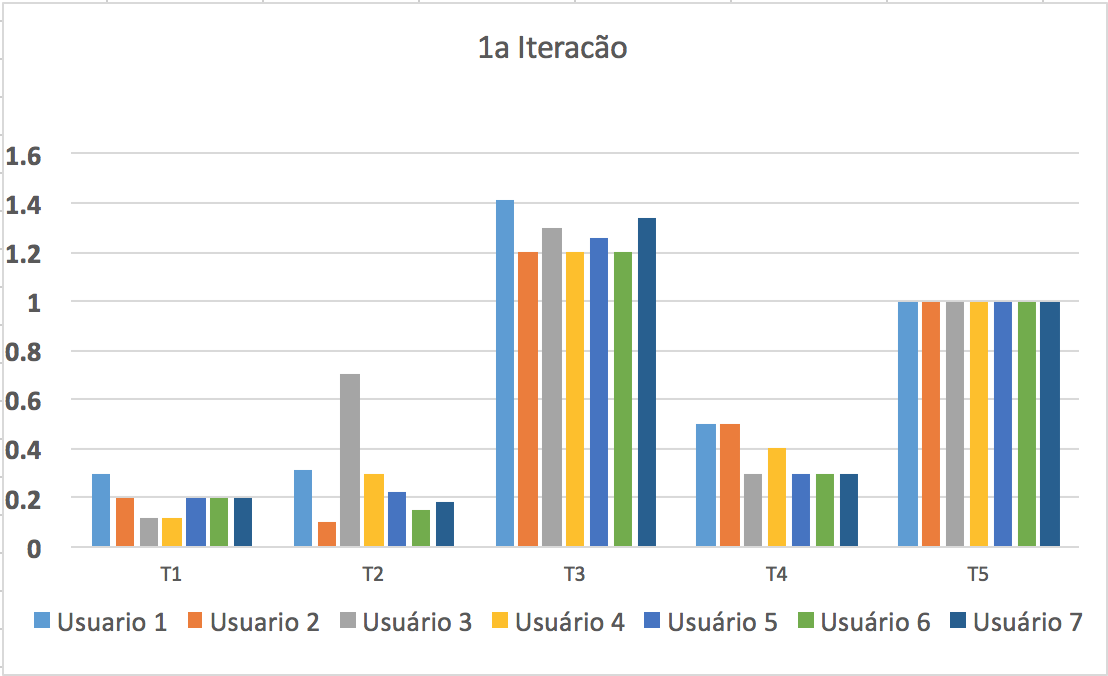
\includegraphics[scale=0.75]{iteracao1_grafico}
\caption{Gráfico Comparativo das Atividades Realizadas na Iteração 1}
\label{img:grafico_iteracao1}
\end{figure}

\begin{table}[h!]
\centering
\caption{Tempo de Execução de Cada Atividade em Segundos 1a Iteração}
\label{tabela_iteracao1}
\begin{tabular}{|llllll|}
\hline
\multicolumn{6}{|c|}{\cellcolor[HTML]{C0C0C0}\textbf{1a Iteracão}}                     \\ \hline
                   & \textbf{T1} & \textbf{T2} & \textbf{T3} & \textbf{T4} & \textbf{T5} \\ \hline
\textbf{Usuário 1} & 0.3         & 0.31        & 1.41        & 0.5         & 1           \\ \hline
\textbf{Usuário 2} & 0.2         & 0.1         & 1.2         & 0.5         & 1           \\ \hline
\textbf{Usuário 3} & 0.12        & 0.7         & 1.3         & 0.3         & 1           \\ \hline
\textbf{Usuário 4} & 0.12        & 0.3         & 1.2         & 0.4         & 1           \\ \hline
\textbf{Usuário 5} & 0.2         & 0.22        & 1.26        & 0.3         & 1           \\ \hline
\textbf{Usuário 6} & 0.2         & 0.15        & 1.2         & 0.3         & 1           \\ \hline
\textbf{Usuário 7} & 0.2         & 0.18        & 1.34        & 0.3         & 1           \\ \hline
\end{tabular}
\end{table}


Após as atividades propostas pelo entrevistador, perguntava-se aos entrevistados quanto à experiencia que eles haviam tido ao utilizar o software. Um dos pontos ressaltados pelos entrevistados foi quanto ao uso de não haver uma descrição quanto a funcionalidade de voltar ao menu utilizando o canto esquerdo superior da tela como pode ser observado na Figura \ref{img:alteracao_menu}. 

\graphicspath{{figuras/}}
\begin{figure}[h!]
\centering
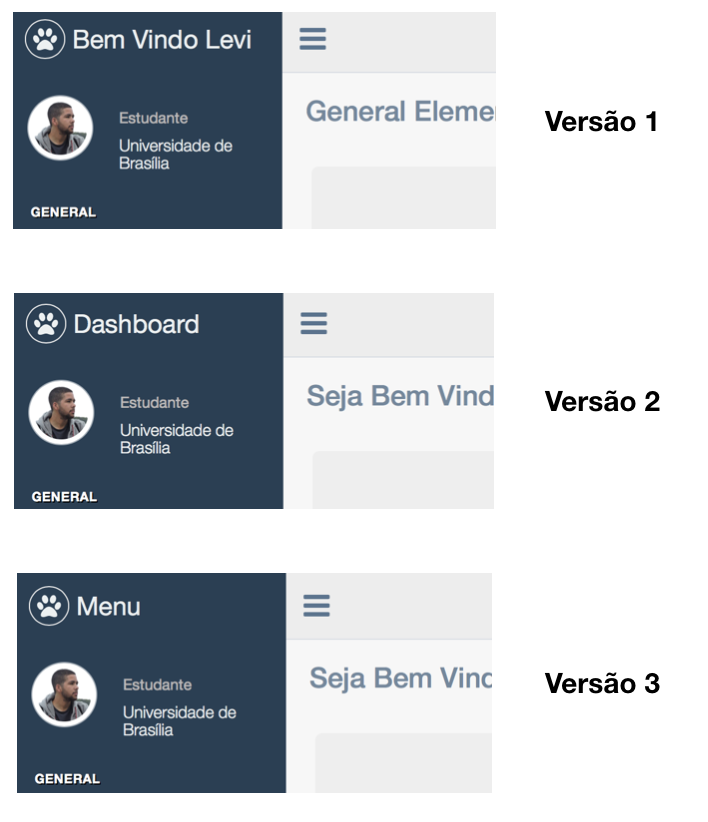
\includegraphics[scale=0.80]{comparacao_versoes_menu}
\caption{Alterações feitas no \textit{link} de menu}
\label{img:alteracao_menu}
\end{figure}

Para a segunda \textit{sprint} decidiu-se elaborar as funcionalidades de acompanhar projeto e exibir métricas. Foram entrevistadas as mesmas pessoas da primeira Iteração e seguiu-se as mesmas atividades da Iteração anterior. Os resultados obtidos estão na Tabela \ref{tabela_iteracao2}. A partir do gráfico presente na Figura \ref{img:grafico_iteracao2} percebe-se que o Usuário 1 apresentou um comportamento fora do esperado, isso se deve ao fato de que o examinado havia se confundido quanto ao enunciado da Tarefa 5.


\begin{table}[h!]
\centering
\caption{Tempo de Execução de Cada Atividade em Segundos 2a Iteração}
\label{tabela_iteracao2}
\begin{tabular}{|llllllll|}
\hline
\multicolumn{8}{|c|}{\cellcolor[HTML]{C0C0C0}\textbf{2a Iteração}}                                                   \\ \hline
                   & \textbf{T1} & \textbf{T2} & \textbf{T3} & \textbf{T4} & \textbf{T5} & \textbf{T6} & \textbf{T7} \\ \hline
\textbf{Usuário 1} & 0.04        & 0.32        & 0.11        & 0.19        & 0.37        & 0.07        & 0.07        \\ \hline
\textbf{Usuário 2} & 0.05        & 0.2         & 0.07        & 0.16        & 0.07        & 0.32        & 0.05        \\ \hline
\textbf{Usuário 3} & 0.05        & 0.17        & 0.05        & 0.14        & 0.08        & 0.27        & 0.02        \\ \hline
\textbf{Usuário 4} & 0.04        & 0.2         & 0.02        & 0.13        & 0.08        & 0.3         & 0.04        \\ \hline
\textbf{Usuário 5} & 0.05        & 0.22        & 0.12        & 0.15        & 0.07        & 0.35        & 0.05        \\ \hline
\textbf{Usuário 6} & 0.05        & 0.24        & 0.16        & 0.16        & 0.07        & 0.26        & 0.05        \\ \hline
\textbf{Usuário 7} & 0.06        & 0.2         & 0.16        & 0.18        & 0.07        & 0.05        & 0.06        \\ \hline
\end{tabular}
\end{table}

\graphicspath{{figuras/}}
\begin{figure}[h!]
\centering
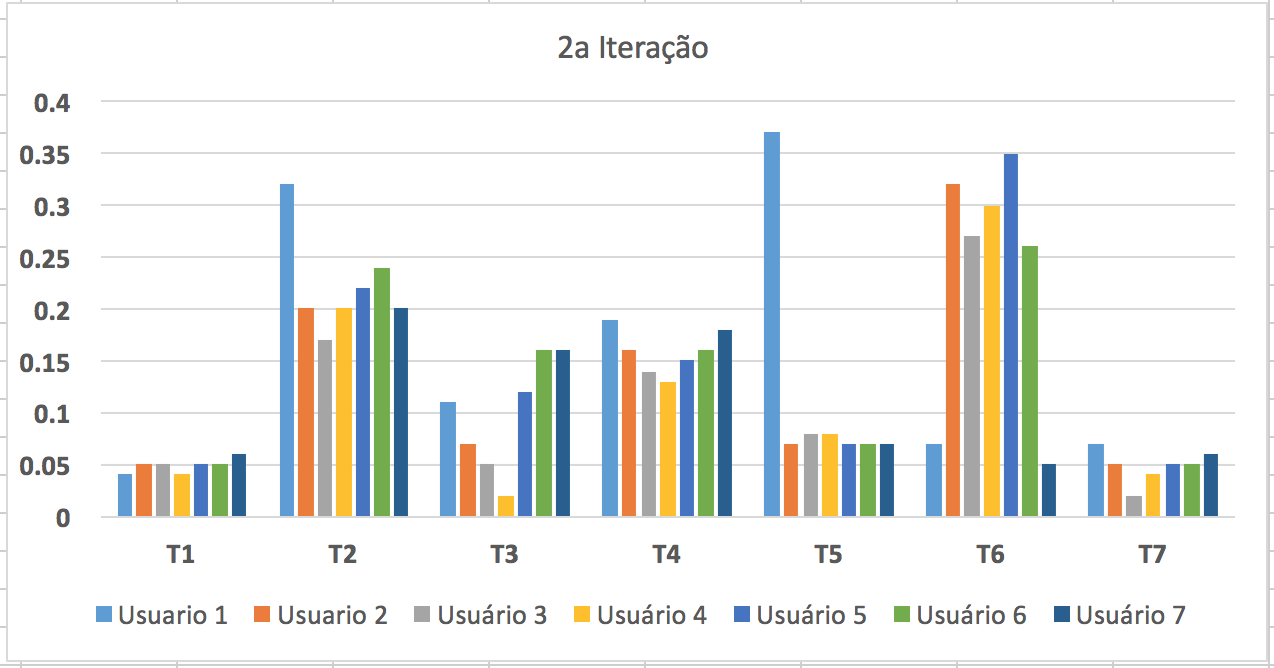
\includegraphics[scale=0.75]{grafico_2a_iteracao}
\caption{Gráfico Comparativo das Atividades Realizadas na Iteração 2}
\label{img:grafico_iteracao2}
\end{figure}

 Uma das mudanças implementadas nessa segunda iteração se deve ao acréscimo de um botão para adicionar projeto na própria pagina inicial da aplicação. Este pedido havia sido feito na 1a Iteração por um dos entrevistados. Está alteração pode ser vista na Figura \ref{img:compara_botao}.
 
 
 \graphicspath{{figuras/}}
 \begin{figure}[h!]
 \centering
 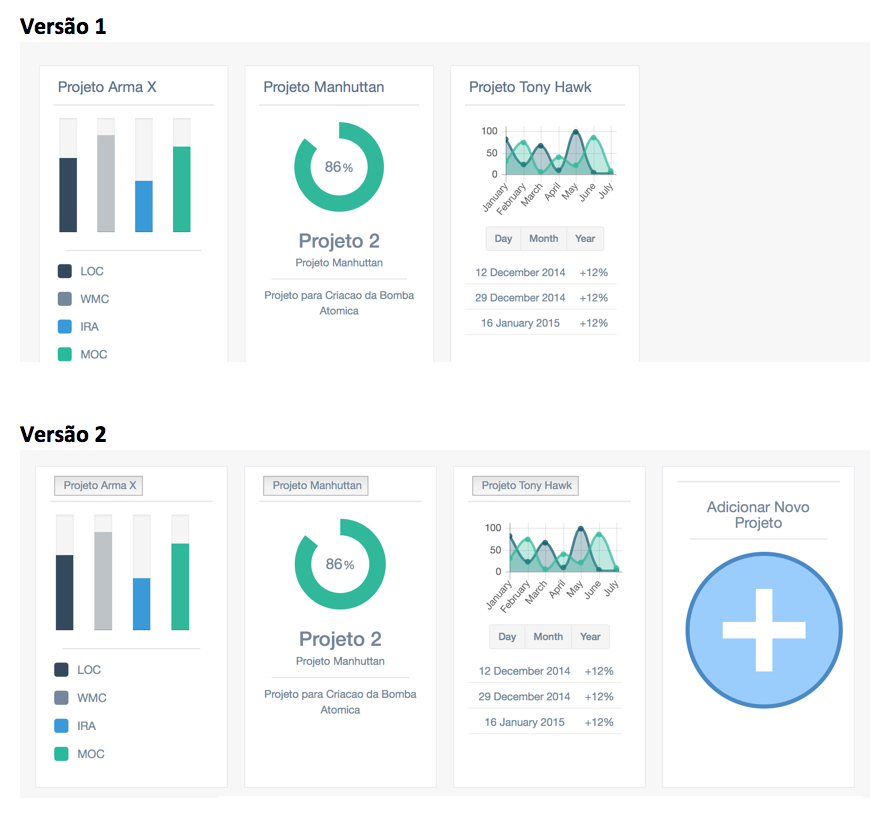
\includegraphics[scale=0.60]{compara_adicao_botao}
 \caption{Acréscimo do Botão de Adicionar Projeto na Página Inicial}
 \label{img:compara_botao}
 \end{figure}
 

A terceira e última \textit{sprint} consistia na implementação da funcionalidade de Criar Módulo de Sugestão de Métricas. Para implementar essa função optou-se pela implementação de uma solução em Python que compara o perfil do gestor que está cadastrando um projeto com outros quatro perfis de gestores. Devido ao fato de não ter havido interesse por parte de gestores reais, optou-se pelo uso de Personas para simular os quatro gestores. A primeira persona criada é o Gestor 1. Gestor 1 possui um perfil mais voltado para gestores que preferem o excesso de métricas à insuficiencia de informação. A segunda \textit{Persona} é o Gestor 2. O perfil do Gestor 2 é mais parecido com o de um gestor mais inexperiente e que não sabe ainda ao certo quais métricas são mais importantes, por isso o valor alto na maioria das métricas escolhidas. O Gestor 3 possui um perfil voltado para gestores que só desejam as informações essenciais, as métricas desse perfil tendem a ser métricas que impactam diretamente na usabilidade da ferramenta. Por último, o Gestor 4 é uma simulação de um gestor que é inexperiente e ao mesmo tempo não conhece muitas das métricas e por isso avalia somente as que conhece. A Figura X ilustra um quadro com as métricas e as notas das métricas dada por cada \textit{Persona}. 


COLOCAR FIGURA




As Figuras seguintes apresentam o estado final da aplicação. Na Figura \ref{img:pag_inicial} destaca-se o botão para acesso rápido ao cadastro de um novo projeto, que foi um dos pontos levantados pelos entrevistados. Outro destaque desta figura está nos \textit{widgets} personalizaveis que apresentam uma visão resumida do estado atual do projeto.

\graphicspath{{figuras/}}
\begin{figure}[h!]
\centering
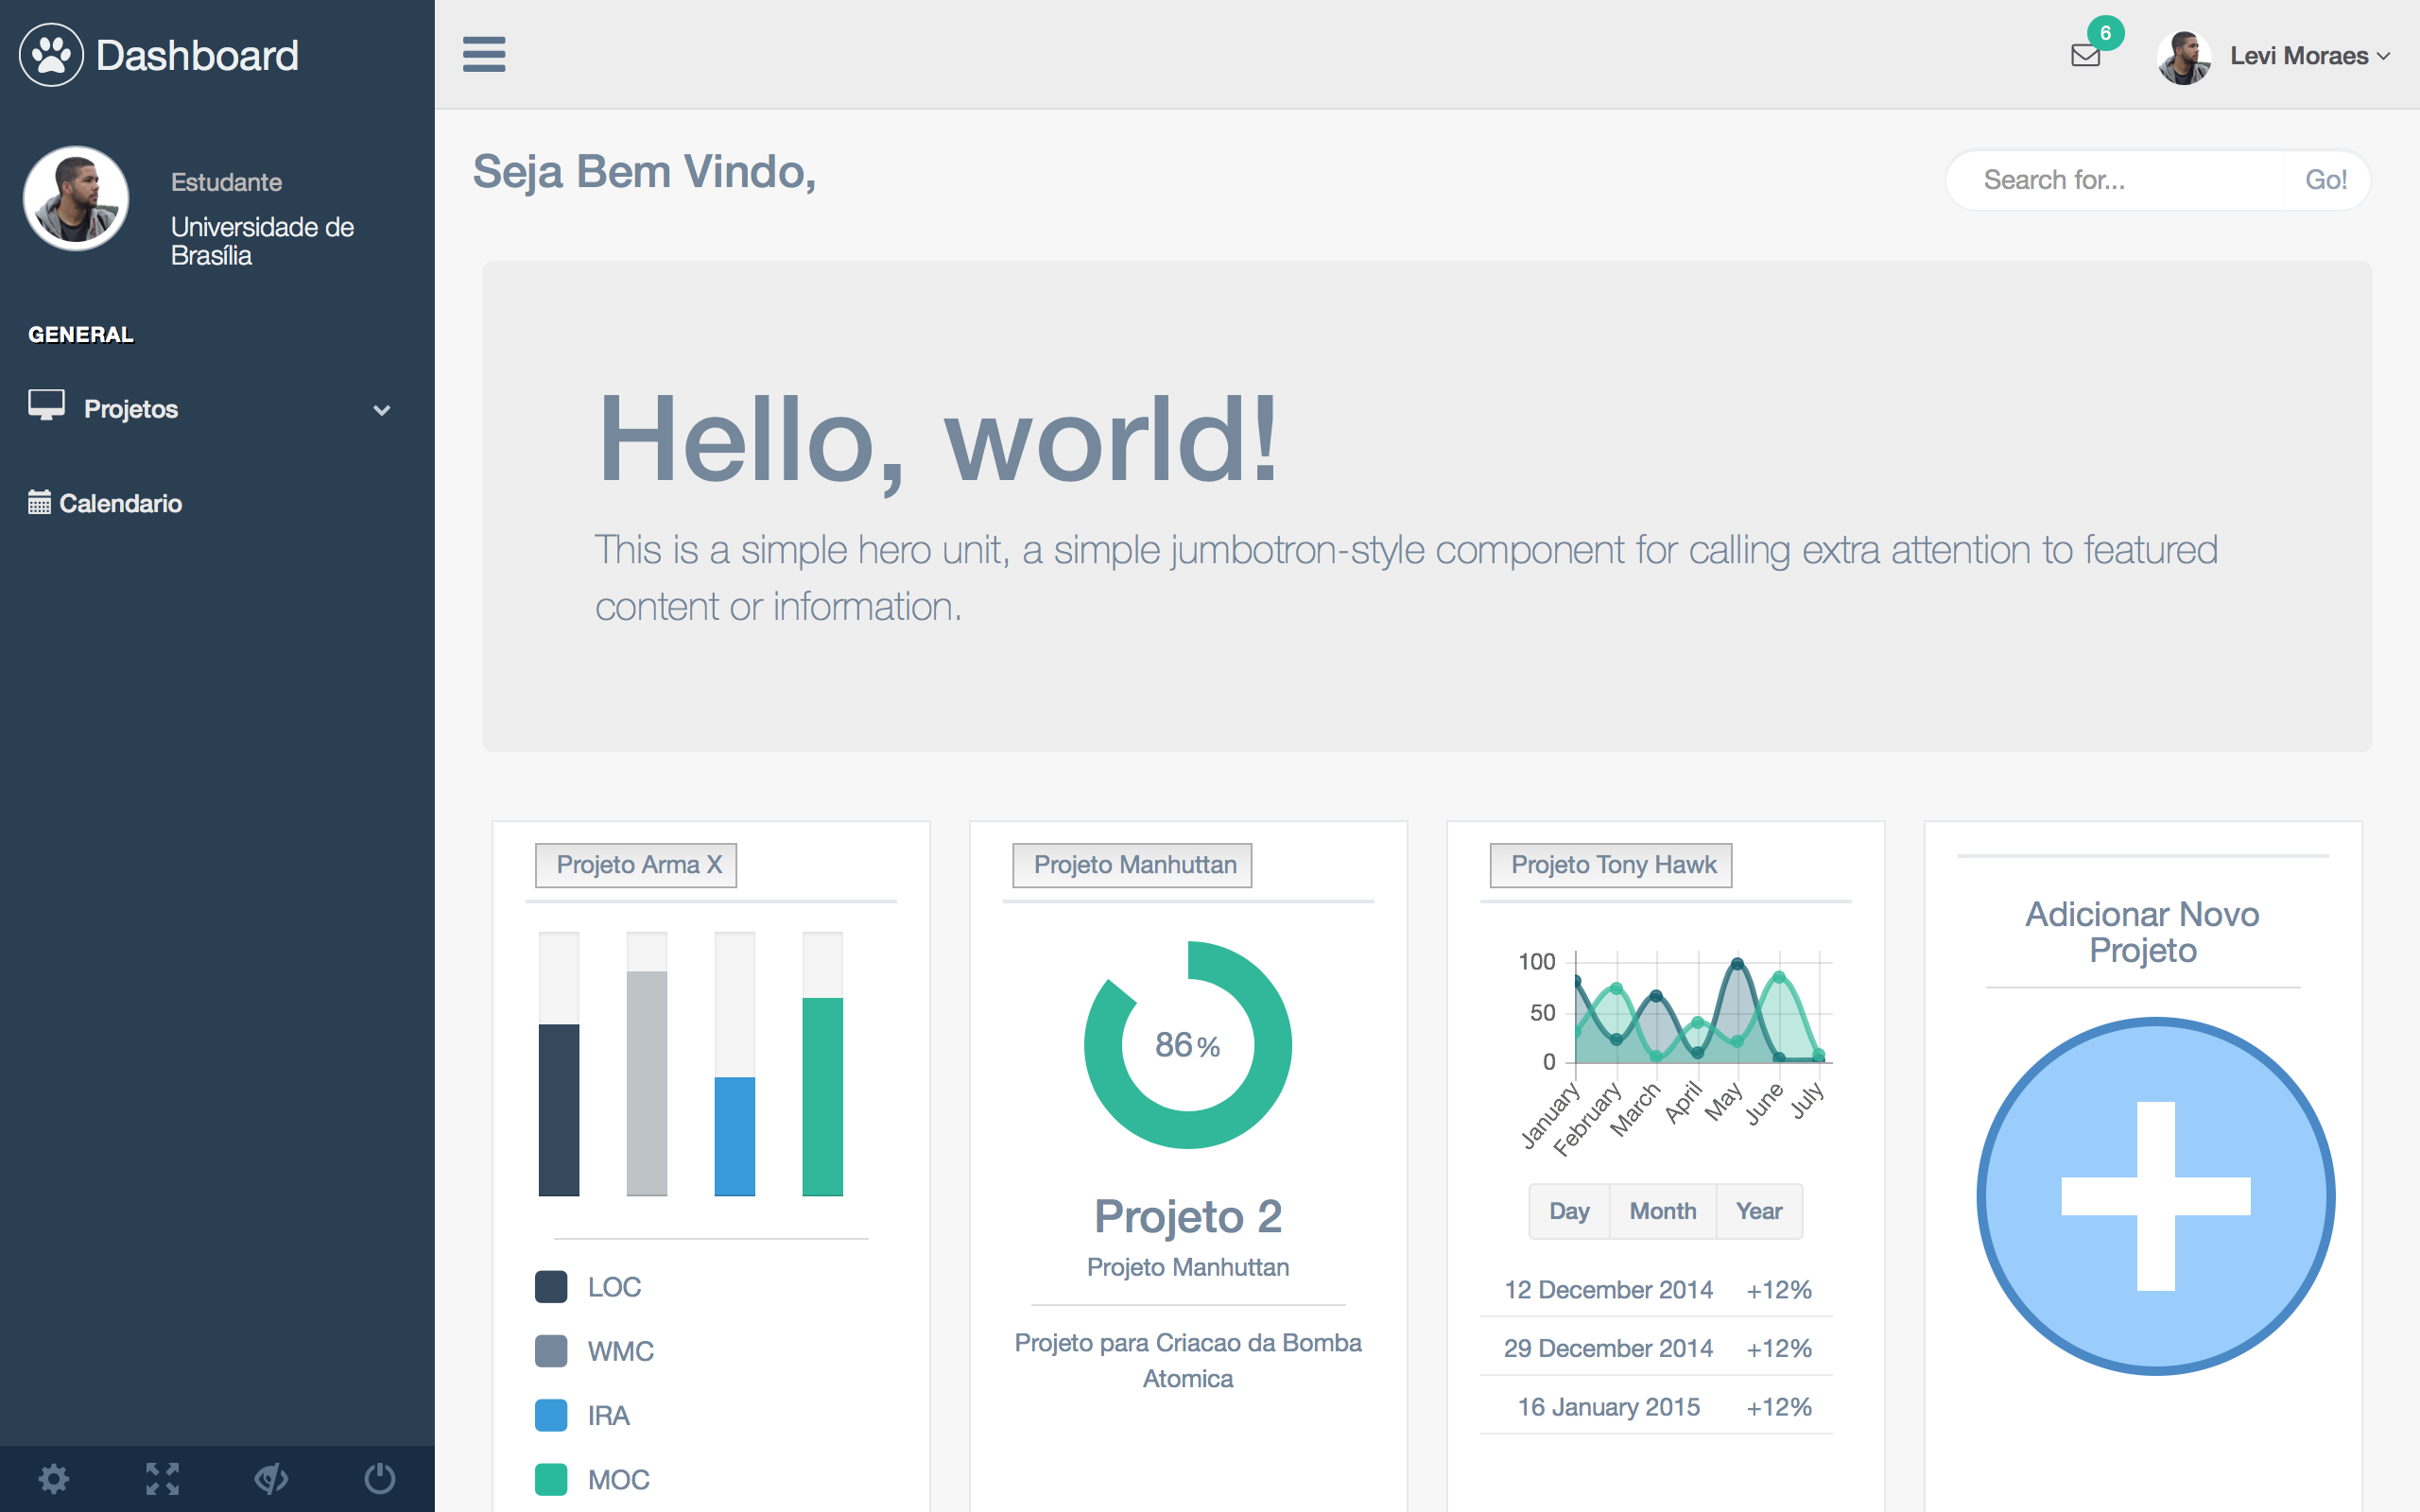
\includegraphics[scale=0.35]{pagina_inicial}
\caption{Página Inicial da Aplicação}
\label{img:pag_inicial}
\end{figure}

A Figura \ref{img:pag_visual} apresenta todos os projetos do gestor, indicando o status de completude do projeto em relação à data de entrega. Percebe-se também a utilização de ícones para representar ações comuns e ja conhecidas do usuário, como o lápis indicando que aquele botão refere-se ao alterar, e a lixeira indicando a ação de exclusão. Ressalta-se também o uso das cores nos botões, em que ações destrutivas (como a deleção de um projeto), apresenta uma cor de destaque em relação as demais.


\graphicspath{{figuras/}}
\begin{figure}[h]
\centering
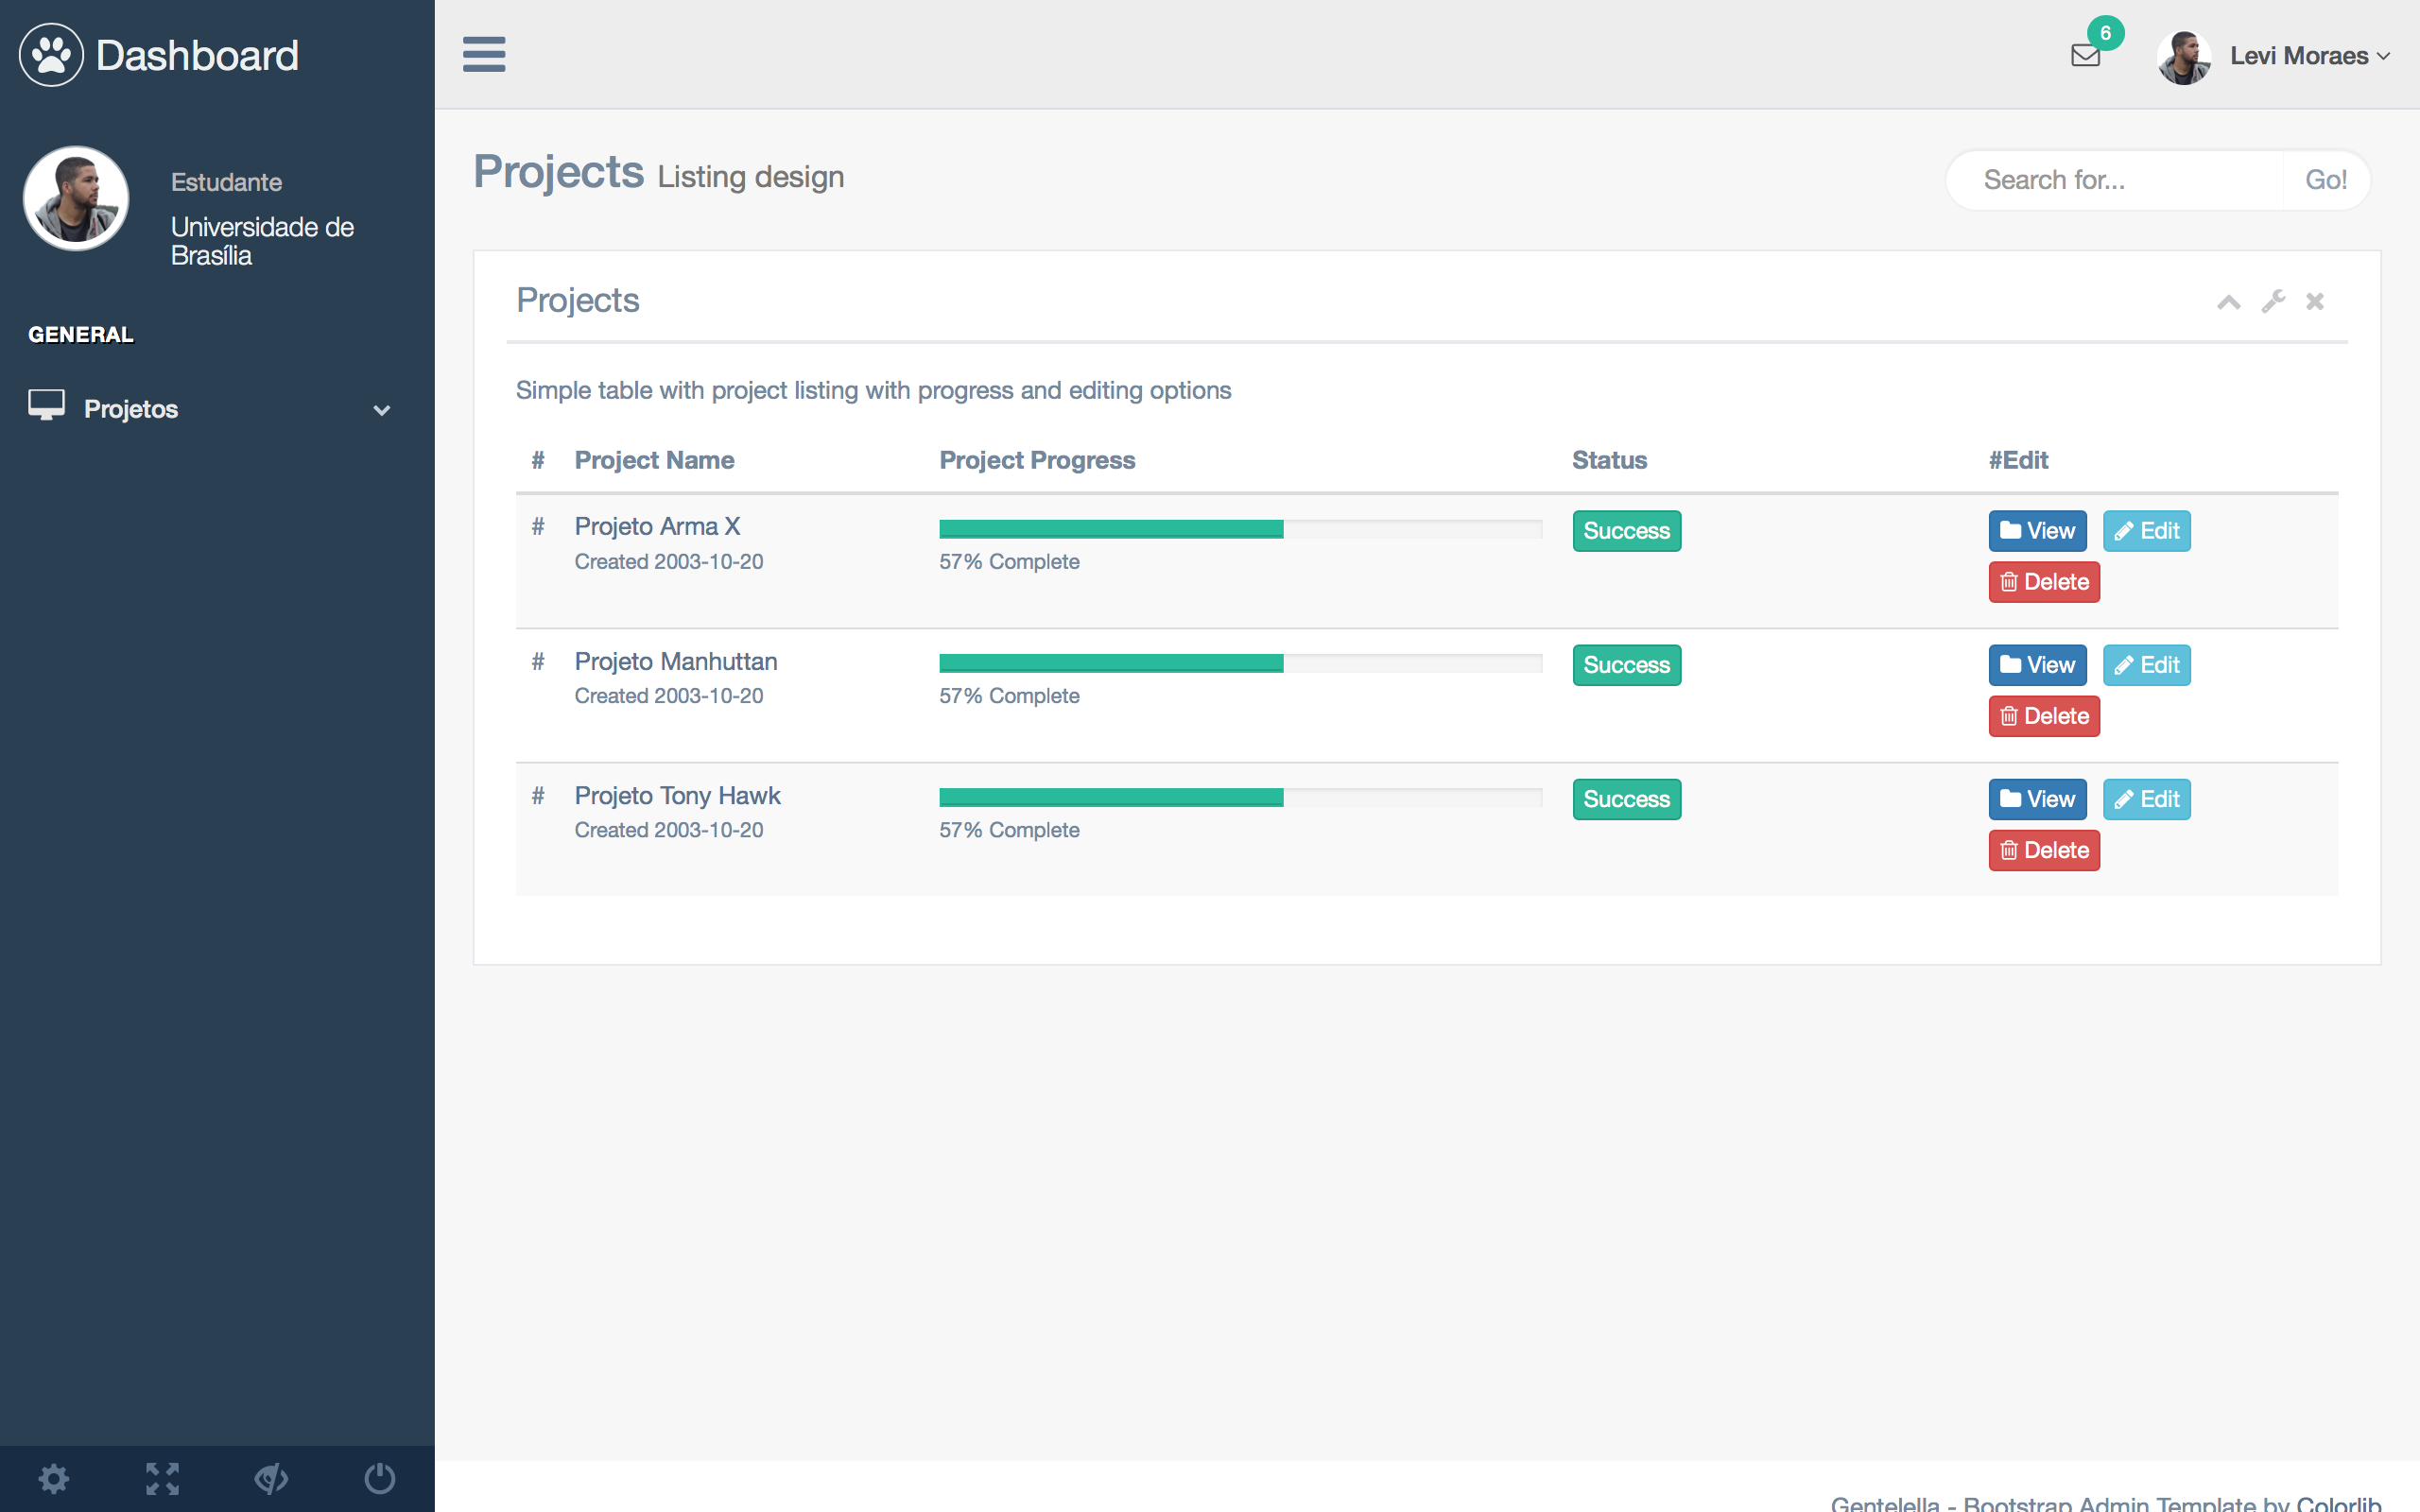
\includegraphics[scale=0.35]{visualizacao_projetos}
\caption{Página de Visualização de Projetos}
\label{img:pag_visual}
\end{figure}

A Figura \ref{img:pag_calendario} apresenta uma funcionalidade que foi sugerida por um dos entrevistados. Está funcionalidade não havia sido planejada inicialmente, mas por ser uma possível necessidade de um cliente, optou-se pela implementação. 

\graphicspath{{figuras/}}
\begin{figure}[h]
\centering
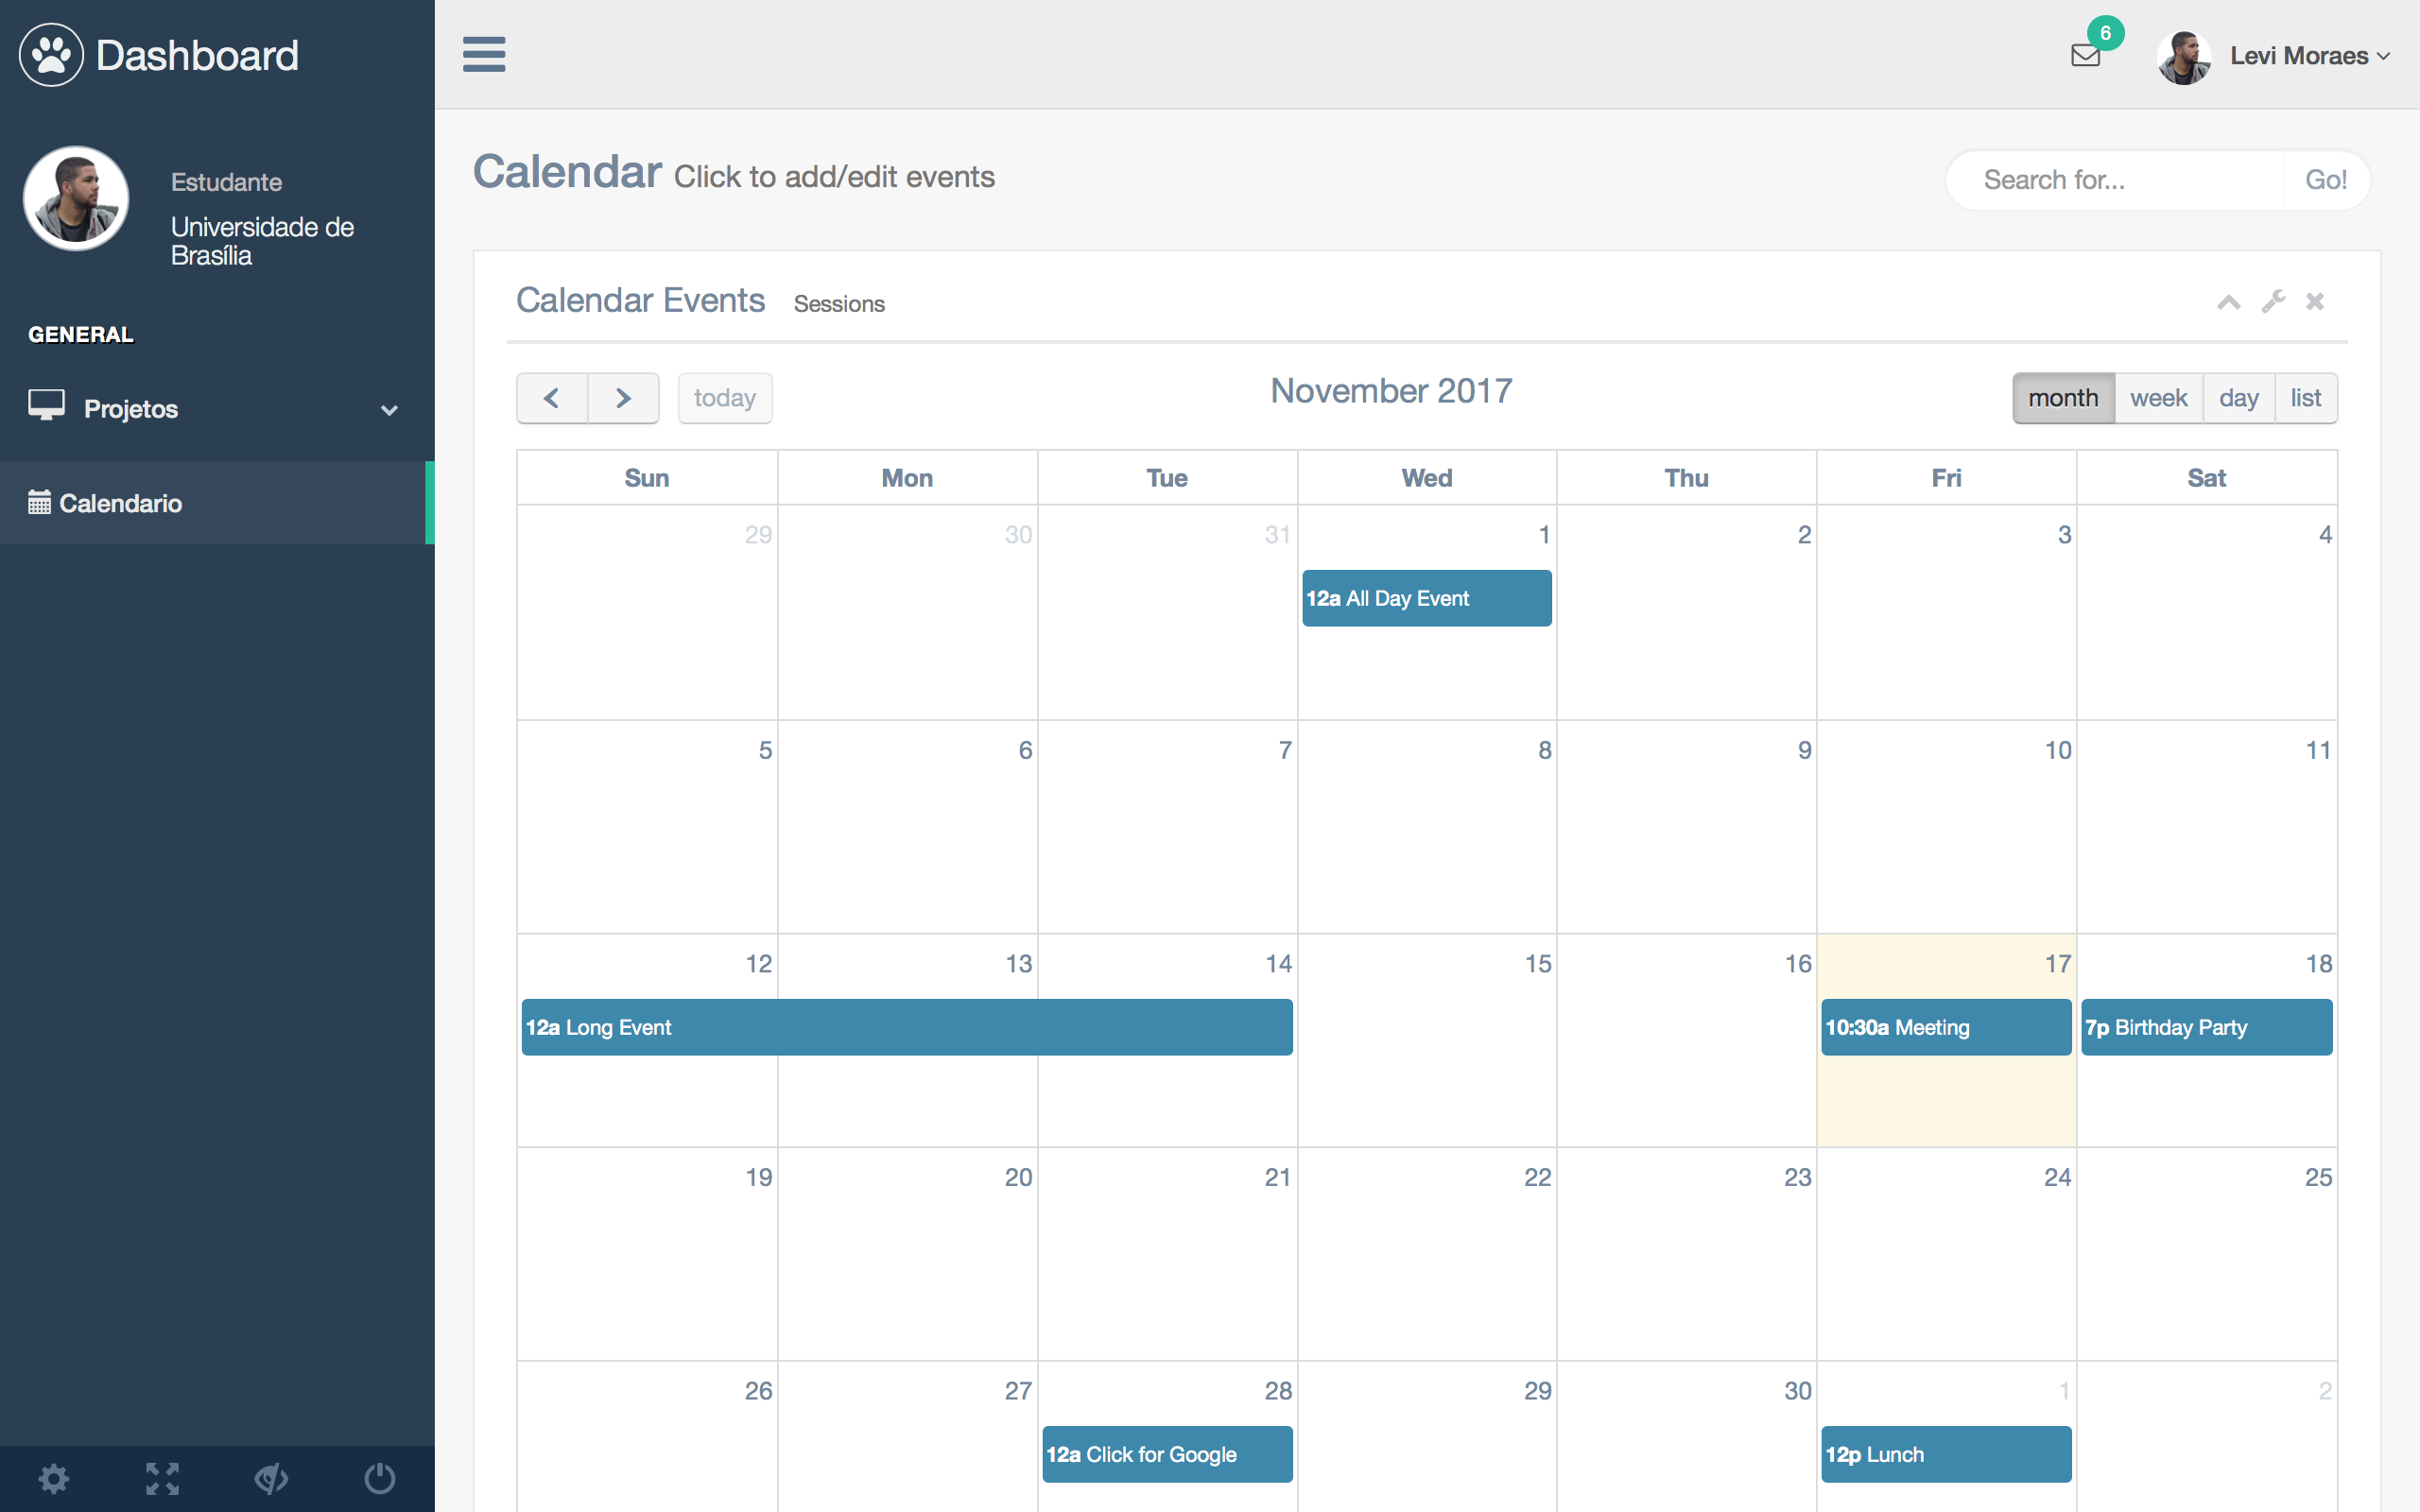
\includegraphics[scale=0.35]{calendario}
\caption{Página de Calendário da Aplicação}
\label{img:pag_calendario}
\end{figure}


A Tabela \ref{table_status} apresenta os \textit{status} de completude do trabalho. Quase todas as atividades foram realizadas, apenas as atividades de Acompanhar Utilização do Software e Aplicar Questionário não foram realizadas. A não realização das atividades se deve ao fato de que não foi possível a implantação da ferramenta em um ambiente real e por consequência não foi possível avaliar a eficácia da ferramenta.


\begin{table}[h!]
\centering
\label{table_status}
\begin{tabular}{lc}
\rowcolor[HTML]{9A0000} 
{\color[HTML]{FFFFFF} \textbf{Atividade}} & \multicolumn{1}{l}{\cellcolor[HTML]{9A0000}{\color[HTML]{FFFFFF} \textbf{Status}}} \\ \hline
Definir Tema                              & 100\%                                                                              \\ \hline
Validar Escopo                            & 100\%                                                                              \\ \hline
Elaborar Roteiro de Pesquisa              & 100\%                                                                              \\ \hline
Pesquisar Referência                      & 100\%                                                                              \\ \hline
Refinar Pesquisa                          & 100\%                                                                              \\ \hline
Catalogar Material                        & 100\%                                                                              \\ \hline
Documentar                                & 100\%                                                                               \\ \hline
Analisar Ambiente                         & 100\%                                                                               \\ \hline
Configurar Ambiente                       & 100\%                                                                                \\ \hline
Implementar Solução de Software           & 100\%                                                                                \\ \hline
Implantar Solução em Ambiente Simulado    & 100\%                                                                                \\ \hline
Acompanhar Utilização do Software         & 0\%                                                                                \\ \hline
Aplicar Questionário                      & 0\%                                                                                \\ \hline
\end{tabular}
\end{table}


\section{Conclusão}

A escolha das métricas para análise, avaliação e acompanhamento de um software, é parte importante quando se fala de contratação de software. Contudo, a escolha das métricas é uma atividade muito subjetiva para que se possa definir contextos e situações específicas para um determinado grupo de métricas. A capacidade de avaliar as melhores métricas para determinados projetos veêm com a experiencia, por isso gestores mais antigos tendem a usar métricas mais específicas para cada projeto. 
Através deste trabalho, pode-se observar a carencia do mercado em soluções de software que auxiliam os gestores nas tomadas de decisões, principalmente no que diz respeito à qualidade de código. Deve-se ressaltar também que o "engessamento" e a comodidade dentro dos órgãos, dificultam a implantação de novas tecnologias.
Uma possível idéia de trabalho derivado deste, seria um estudo de caso avaliando a implantação do software produzido em um órgão real, e acompanhar o quão relevante a ferramenta se mostrou nas licitações de software.